\documentclass[french]{beamer}

\usepackage[utf8]{inputenc}
\usepackage[T1]{fontenc}
\usepackage{lmodern}
\usepackage{amsmath, amssymb}
\usepackage{graphicx} 
\graphicspath{ {screenshoot} }

\usepackage{babel}

%CHOIX DU THEME et/ou DE SA COULEUR
% => essayer différents thèmes (en décommantant une des trois lignes suivantes)
\usetheme{PaloAlto}
%\usetheme{Madrid}
%\usetheme{Copenhagen}

% => il est possible, pour un thème donné, de modifier seulement la couleur
%\usecolortheme{crane}
% \usecolortheme{seahorse}

% \useoutertheme[left]{sidebar}


%Pour le TITLEPAGE
\title[QA to NL]{Question Answering to Natural Languages}
\subtitle{Cours : Tatia}
\author[FD et VA]{Fissore et Venturelli}
\date{Année 2021-2022}
\institute[UCA]{Université Côte d'Azure -- M1 Informatique}

\addtobeamertemplate{navigation symbols}{}{%
  \usebeamerfont{footline}%
  \usebeamercolor[fg]{footline}%
  \hspace{1em}%
  \insertframenumber/\inserttotalframenumber
}


\begin{document}

\begin{frame}
  \titlepage
\end{frame}

\begin{frame}
  Un environnement \texttt{frame} pour chaque \emph{diapositive}.
  \visible<2>{Chaque diapo pouvant contenir plusieurs \emph{couches}.}
\end{frame}


\begin{frame}{Sommaire}
  \tableofcontents
\end{frame}

\section{Introduction}
% Ici on parle de la repartition des taches, 
% du pourquoi on a choisi ce sujet
\begin{frame}{Pourquoi notre projet ?}
  blabla
  %au debut on savait pas quoi faire ...
  \begin{figure}[htbp]
    \centerline{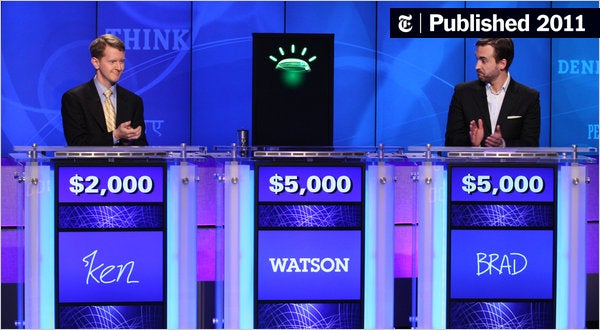
\includegraphics[scale=0.3]{watson.jpg}}
    \caption{Watson at Jeopardy Quiz}
  \end{figure}
\end{frame}

\begin{frame}
  Un \textbf<2,3>{texte} en gras.
  \visible<3>{Un texte visible sur la 3\ieme{} couche}
\end{frame}

\begin{frame}{Titre (facultatif)}
  \framesubtitle{Sous titre (facultatif aussi)}
  \begin{block}{Remarque}
    Un bloc
  \end{block}

  \begin{alertblock}{Proposition}
    Un bloc alerte
  \end{alertblock}

  \begin{exampleblock}<2>{Exemple}
    Un bloc exemple qui est visible sur la 2\ieme{} couche : $f(x)=2x$.
  \end{exampleblock}
\end{frame}

\section{Section 2}
\begin{frame}{La section 2 commence}
  \begin{itemize}
    \item<1-> On peut cliquer sur les titres de la barre de gauche pour naviguer dans les sections du pdf (essayez !).
    \item<2-> On peut changer le ``look'' du beamer, en changeant de thème. Retournez dans le fichier source et compilez avec les autres thèmes proposés (il existe énormément de thèmes; seuls trois sont proposés dans le source).
  \end{itemize}

\end{frame}

\section{Dataset}
\begin{frame}{Title}
  blabla
\end{frame}

\section{Parseur}
\begin{frame}{Title}
  blabla
\end{frame}

\section{Parcours de l'arbre}
\begin{frame}{Title}
  blabla
\end{frame}

\section{Analyse des resultats}
\begin{frame}
  bla
\end{frame}

\section{Conclusions}
\begin{frame}
  bla
\end{frame}

\end{document}